\documentclass[10pt,a4paper]{ltjsarticle}       % LuaTeX を使う
\usepackage[luatex]{graphicx}             % LuaTeX 用, draft がついているときは図の代わりに同じ大きさの枠ができる
\usepackage{here}                               % 図表の位置を強制して出力
\usepackage{afterpage}                          % 残っている図を貼り付ける(\afterpage{\clearpage})
\usepackage[subrefformat=parens]{subcaption}    % サブキャプション(図1(a) とか)
\usepackage{setspace}                           % 行間制御
\usepackage{ulem}                               % 下線や取り消し線など
\usepackage{booktabs}                           % きれいな表(\toprule \midrule \bottomrule)
\usepackage{multirow}                           % 表で行結合
\usepackage{multicol}                           % 表で列結合
\usepackage{hhline}                             % 表で 2 重線
\usepackage[table]{xcolor}                      % カラー
\usepackage{tikz}                               % 図描画用
\usepackage[framemethod=tikz]{mdframed}         % 文章を囲むとき用
\usepackage[version=3]{mhchem}                  % 化学式
\usepackage{siunitx}                            % 単位
\usepackage{comment}                            % コメント
\setcounter{tocdepth}{3}                        % 目次に subsubsection まで表示
% -----ヘッダ・フッタの設定-----
\usepackage{fancyhdr}
\usepackage{lastpage}
\pagestyle{fancy}
\lhead{}                                 % 左ヘッダ
\chead{}                                 % 中央ヘッダ
\rhead{}                                 % 右ヘッダ
\lfoot{}                                 % 左フッタ
\cfoot{\thepage~/~\pageref{LastPage}}    % 中央フッタ
\rfoot{}                                 % 右フッタ
\renewcommand{\headrulewidth}{0pt}       % ヘッダの罫線を消す
% -----余白の設定-----
% これをアンコメントするとページ番号が中央からずれるから今は使わない.
% \usepackage[left=19.05mm,right=19.05mm,top=25.40mm,bottom=25.40mm]{geometry}
% -----フォントの設定-----
% https://ja.osdn.net/projects/luatex-ja/wiki/LuaTeX-ja%E3%81%AE%E4%BD%BF%E3%81%84%E6%96%B9
% http://myfuturesightforpast.blogspot.jp/2013/12/tex-gyre.html など
\usepackage[no-math]{fontspec}
\usepackage{amsmath,amssymb}    % 高度な数式用
\usepackage{mathrsfs}           % 花文字用
% times ベース -> txfonts
% palatino ベース -> pxfonts
\usepackage{txfonts}
\usepackage{bm}                 % 斜体太字ベクトル
% Avant Garde -> TeX Gyre Adventor
% Bookman Old Style -> TeX Gyre Bonum
% Zapf Chancery -> TeX Gyre Chorus
% Courier -> TeX Gyre Cursor
% Helvetica -> TeX Gyre Heros
% Helvetica Narrow -> TeX Gyre Heros Cn
% Palatino -> TeX Gyre Pagella
% New Century Schoolbook -> TeX Gyre Schola
% Times -> TeX Gyre Termes
\setmainfont[Ligatures=TeX]{TeXGyreTermes}
\setsansfont[Ligatures=TeX]{TeXGyreHeros}
\setmonofont[Scale=MatchLowercase]{TeXGyreCursor}
\usepackage[match,deluxe,expert,bold]{luatexja-fontspec}
\setmainjfont[BoldFont=IPAexGothic]{IPAexMincho}
\setsansjfont{IPAexGothic}
\usepackage{luatexja-otf}
% -----PDF ハイパーリンク,ブックマーク,URL の設定-----
% オプション(\hypersetup{})は https://texwiki.texjp.org/?hyperref 参照
\usepackage{url}
% -----ソースコードの設定-----
% オプション(\lstset{})は http://tug.ctan.org/tex-archive/macros/latex/contrib/listings/listings.pdf 参照
% 使うときは
% \begin{lstlisting}[language=aaaa,caption=bbbb,label=List:cccc]
% hogehoge
% \end{lstlisting}
\usepackage{listings}
\lstset{%
  basicstyle=\ttfamily\small,%
  frame=single,%
  frameround=ffff,%
  numbers=left,%
  stepnumber=1,%
  numbersep=1\zw,%
  breaklines=true,%
  tabsize=4,%
  captionpos=t,%
  commentstyle=\itshape}
% -----図表等の reference の設定-----
% 表示文字列を日本語化
\renewcommand{\figurename}{図}
\renewcommand{\tablename}{表}
\renewcommand{\lstlistingname}{リスト}
\renewcommand{\abstractname}{概要}
% 図番号等を"<章番号>.<図番号>"
% lstlisting に関しては https://tex.stackexchange.com/questions/134418/numbering-of-listings 参照
\renewcommand{\thefigure}{\thesection.\arabic{figure}}
\renewcommand{\thetable}{\thesection.\arabic{table}}
\AtBeginDocument{\renewcommand{\thelstlisting}{\thesection.\arabic{lstlisting}}}
\renewcommand{\theequation}{\thesection.\arabic{equation}}
% 節が進むごとに図番号等をリセット
% http://d.hatena.ne.jp/gp98/20090919/1253367749 参照
\makeatletter
\@addtoreset{figure}{section}
\@addtoreset{table}{section}
\@addtoreset{lstlisting}{section}
\@addtoreset{equation}{section}
\makeatother
% \ref{} の簡単化
\newcommand*{\refSec}[1]{\ref{#1}~章}
\newcommand*{\refSsec}[1]{\ref{#1}~節}
\newcommand*{\refSssec}[1]{\ref{#1}~項}
\newcommand*{\refFig}[1]{\figurename~\ref{#1}}
\newcommand*{\refTab}[1]{\tablename~\ref{#1}}
\newcommand*{\refList}[1]{\lstlistingname~\ref{#1}}
\newcommand*{\refEq}[1]{式~(\ref{#1})}
% -----数式中便利な定義-----
% https://www.library.osaka-u.ac.jp/doc/TA_LaTeX2.pdf
% https://en.wikibooks.org/wiki/LaTeX/Mathematics など
\newcommand{\e}{\mathrm{e}}                     % ネイピア数
\newcommand{\imagi}{\mathrm{i}}                 % 虚数単位(i)
\newcommand{\imagj}{\mathrm{j}}                 % 虚数単位(j)
\newcommand{\vDel}{\varDelta}                   % デルタ大文字
\newcommand{\veps}{\varepsilon}                 % イプシロン小文字
\newcommand*{\paren}[1]{\left( #1 \right)}      % () を中身の大きさに合わせる
\newcommand*{\curly}[1]{\left\{ #1 \right\}}    % {} を中身の大きさに合わせる
\newcommand*{\bracket}[1]{\left[ #1 \right]}    % [] を中身の大きさに合わせる
\renewcommand{\Re}{\operatorname{Re}}           % 実部
\renewcommand{\Im}{\operatorname{Im}}           % 虚部
\newcommand*\sfrac[2]{{}^{#1}\!/_{#2}}          % xfrac パッケージの \sfrac{}{} の代わり
\renewcommand*\vec[1]{\mathbf{#1}}              % 矢印ベクトルは使わないので上書き.太字立体.

\title{知的システム構成論課題\\矢入先生担当分}
\author{航空宇宙工学専攻修士一年\\37-186305 荒居秀尚}

\begin{document}
\maketitle
\section{選択したテーマ}
今回の課題に向けて選択したテーマは「隠れマルコフモデルとEMアルゴリズムを用いた音声データの潜在状態の推定」としました。
音声データとしては、研究室の研究会の様子を録音したもの、約160分程度のものの一部を使用し、潜在状態として話者
を分類することを目的として学習を行いました。今回のデータはサイズが大きかったのとノイズが多い区間が多かったため
実際のモデルの学習には先述のデータから10秒程度を切り出したものを用い、その検証にも別の区間から10秒程度
切り出したものを使用しました。なお、学習用データに含まれるのは3人分の音声であり、検証用データに含まれるのは
学習用データに含まれていた声のうち2人分でそれ以外の声は含まれていません。このことを考慮して、今回はクラスタ
数を3として事前に与えました。\\

このテーマを選択した理由として、個人的に以前から研究会の文字起こしをしたいと考えており、特に話者を識別して
アノテーションを加えたいという目的がありました。今回はそれをHMMを用いて出来ないか試してみたという例になります。
\section{学習手順}
音声データを扱うにあたって、メル周波数ケプストラム係数(MFCC)に変換を行いました~\cite{soundrecognition}。
MFCCに変換する手順は本質的ではありませんが学習を行うにあたって問題の原因となっていると感じたため記載します。\\

MFCCに変換する手順は以下の6ステップからなります。
\begin{enumerate}
  \item 広域強調
  \item 音声フレーム
  \item STFT
  \item メルフィルタバンクの作成
  \item ケプストラム特徴量の抽出
  \item リフタリング
\end{enumerate}
広域強調は人間の聴覚特性に合わせて広域のパワーを補償する作業です。その後ハミング窓などの窓関数を使って
音声フレームを切り出し、短時間フーリエ変換を行います。その後メル尺度に合わせた特徴量セットを作成して、それを
フーリエ変換後のデータに適用して逆離散コサイン変換をかけることでケプストラム特徴量を得ます。最後にこのケプストラム
特徴量のうち目的に合わせて特徴量を選択します。\\

今回は最後のリフタリングにおいて20次元までに特徴量セットを絞りました。これをGaussianHMMにEMアルゴリズム
を用いて学習させることで、クラスタリングを行います。
\section{結果・考察}
今回は時間がなかったため、アルゴリズム等のスクラッチ実装は行わず、ライブラリ関数を用いただけになってしまったのですが
上記の手順を実装しました。MFCCの抽出はlibrosa\cite{librosa}を用い、GaussianHMMはhmmlearn\cite{hmmlearn},
とbnpy\cite{bnpy}を試しました。結果としては、検証用データには二人分の声しか含まれていないにもかかわらず
クラスタリングのうえでは3クラスへ分類が行われていたため、おそらく発言した人物ごとのクラスタリングは失敗している
と考えられます。以下ではこの原因に関して考察を行います。\\

まず、MFCCの可視化ですが、以下の図\ref{fig:mfcc}のようになりました。
\begin{figure}[htbp]
  \begin{center}
    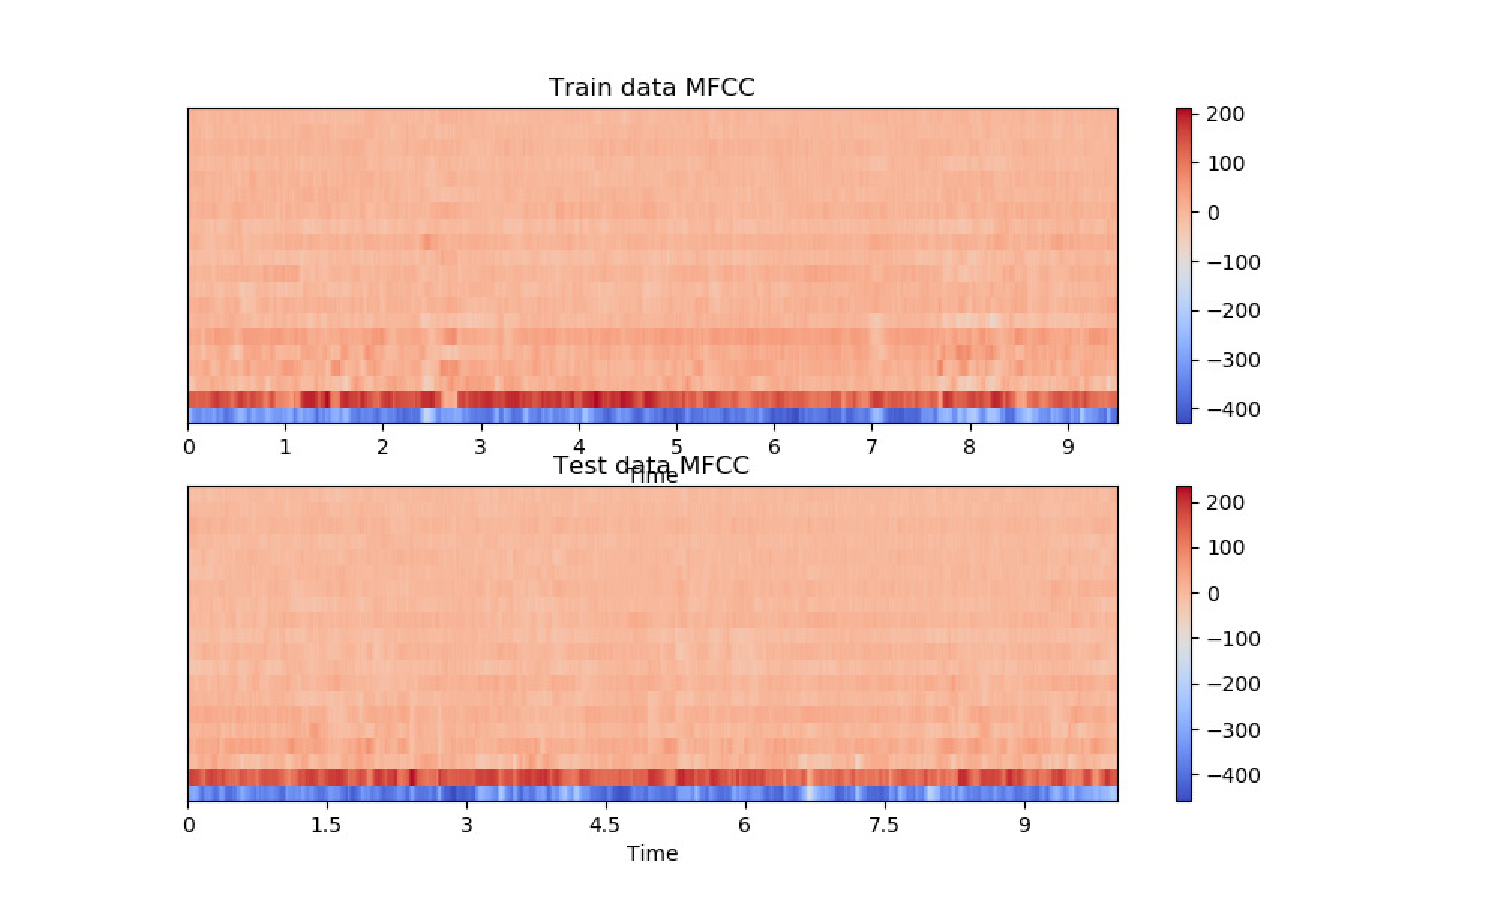
\includegraphics[clip, scale=0.6]{mfcc-eps-converted-to}
    \caption{TrainデータとTestデータをMFCCに変換した結果}
    \label{fig:mfcc}
  \end{center}
\end{figure}
下から順に、MFCCの1番目の成分から20番目の成分が並んでいます。全体として音声パワーが学習データのほうが強く
検証データのほうが弱いものになっていたのですがその影響がやや現れてしまっているように見られます。具体的には
学習データのほうが、2.5秒付近と8秒付近に強い発話があったことに対応する縦に伸びる構造が見えますが、検証
データにはそれほど大きな同様の構造は見られません。また、第6特徴などは学習データでははっきりとした横に伸びる
筋が見られますが、検証データではぼんやりしています。\\

また、bnpyを用いて学習データに対するクラスタリングの結果をクラスタごとのパワーとして表したのが以下の図\ref{fig:power}
です。
\begin{figure}
  \begin{center}
    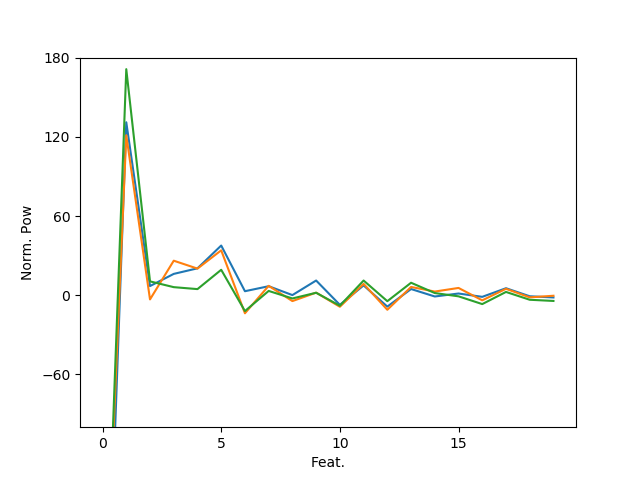
\includegraphics[clip, scale=0.80]{normpVSfeat}
    \caption{Trainデータのクラスタごとのパワー}
    \label{fig:power}
  \end{center}
\end{figure}
この図を見ると第2から第6特徴量に当たる部分が分類に大きく寄与していることがわかります。しかし、個人差が大きい
と言われるのは高ケフレンシー領域、すなわち図\ref{fig:power}の左の方の特徴に集中するため、この部分の違い
をクラスタリングに反映出来ていないことがわかります。この対策は、低ケフレンシー領域を捨てる、ということになりますが
今回は時間が足らずMFCCを自分で実装することが出来なかったためこれは出来ませんでした。\\

また、モデルの面でも今回は、ライブラリを用いるのみとなってしまったため、遷移確率などに制約をかけられなかったことが
1つ失敗の原因と考えられます。今回は学習データが10秒程度と短いため、正確な推論には的確に初期条件を与える
必要があると考えられますが、この部分をしっかりと行わなかったことも原因の1つと考えられます。\\

今後は、この結果を考慮して
\begin{itemize}
  \item MFCCにおいて低ケフレンシー領域の特徴を捨てる
  \item モデルの初期値に対して制約を入れられるようにする
\end{itemize}
といった方向性で音声を人ごとに分離することができると考えられます。
\bibliographystyle{junsrt}
\bibliography{reference}
\end{document}
